\chapter{集合}
\section{元素与集合}
\subsection{集合的概念}
虽然集合是一个原始的概念, 但对一个具体的集合而言, 很多情况下我们还是可以采用列举法或描述法给出它的一个准确而清晰的表示.

用描述法表示一个集合基于下面的概括原则:

概括原则 对任给的一个性质 $P$, 存在一个集合 $S$, 它的元素恰好是具有性质 $P$ 的所有对象, 即

$$
	S=\{x \mid P(x)\}
$$

其中 $P(x)$ 表示 “ $x$ 具有性质 $P "$.

由此,我们知道集合的元素是完全确定的, 同时它的元素之间具有互异性和无序性.

集合的元素个数为有限数的集合称为有限集, 元素个数为无限数的集合称为无限集. 如果有限集 $A$ 的元素个数为 $n$, 则称 $A$ 为 $n$ 元集, 记作 $|A|=n$. 空集不含任何元素.

\begin{example}
	设集合 $M=\left\{x \left\lvert\, \frac{a x-5}{x^{2}-a}<0\right., x \in \mathbf{R}\right\}$. 若 $3 \in M$, 且 $5 \notin M$, 求实数 $a$ 的取值范围.
\end{example}
\begin{solution}
	由 $3 \in M$, 得 $\frac{3 a-5}{3^{2}-a}<0$, 即

	\begin{gather*}
		\left(a-\frac{5}{3}\right)(a-9)>0, \\
		a<\frac{5}{3} \text { 或 } a>9 . \tag{1}
	\end{gather*}


	所以

	由 $5 \notin M$ 得, $\frac{5 a-5}{5^{2}-a} \geqslant 0$ 或 $5^{2}-a=0$, 所以

	\begin{equation*}
		1 \leqslant a \leqslant 25 \tag{2}
	\end{equation*}


	由 (1), (2) 得, $a \in\left[1, \frac{5}{3}\right) \cup(9,25]$.

	说明 $5 \notin M$ 隐含了条件 $5^{2}-a=0$, 这是容易被忽视的.
\end{solution}

\begin{example}
	设集合 $M=\left\{a \mid a=x^{2}-y^{2}, x, y \in \mathbf{Z}\right\}, n$ 为整数. 分别判断数 $4 n ,  4 n+1 ,  4 n+2 ,  4 n+3$ 与集合 $M$ 的关系.
\end{example}

\begin{analysis}
	当 $n=1$ 时, 易知 $4=2^{2}-0^{2}, 5=3^{2}-2^{2}, 7=4^{2}-3^{2}$; 而对任何整数 $x ,  y$, 由于 $x+y$ 与 $x-y$ 同奇偶, 故 $(x+y)(x-y) \neq 2 \times 3=6 \times$ $1=6$. 于是, 我们尝试将 $4 n ,  4 n+1 ,  4 n+3$ 分别表示成 $x^{2}-y^{2}$ 的形式, 并证明不存在 $x, y \in \mathbf{Z}$, 使 $4 n+2=x^{2}-y^{2}$.
\end{analysis}

\begin{solution}
	因为对任意的整数 $n$, 有

	\begin{gather*}
		4 n=(n+1)^{2}-(n-1)^{2}(n+1, n-1 \in \mathbf{Z}) \\
		4 n+1=(2 n+1)^{2}-(2 n)^{2}(2 n+1,2 n \in \mathbf{Z}) \\
		4 n+3=(2 n+2)^{2}-(2 n+1)^{2}(2 n+2,2 n+1 \in \mathbf{Z})
	\end{gather*}

	所以 $4 n, 4 n+1,4 n+3 \in M$.

	若 $4 n+2$ 是 $M$ 的元素, 则存在 $x, y \in \mathbf{Z}$ 满足 $4 n+2=x^{2}-y^{2}$. 注意到 $x+y$ 与 $x-y$ 奇偶性相同, 若同为奇数, 则 $4 n+2=x^{2}-y^{2}=(x+y)(x-$ $y)$ 不成立; 若同为偶数, 则 $(x+y)(x-y)$ 为 4 的倍数, 但 $4 n+2$ 不是 4 的倍数, 故 $4 n+2=x^{2}-y^{2}=(x+y)(x-y)$ 不成立. 所以 $4 n+2$ 不是 $M$ 的元素.

	说明 由概括原则我们知道, 判断一个对象 $x$ 是否为集合 $S$ 的元素, 等价于判断 $x$ 是否具有性质 $P$.
\end{solution}

\begin{example}
	设集合

	$$
		S=\left\{\left.\frac{m+n}{\sqrt{m^{2}+n^{2}}} \right\rvert\, m, n \in \mathbf{N}, m^{2}+n^{2} \neq 0\right\}
	$$

	证明: 对一切 $x, y \in S$, 且 $x<y$, 总存在 $z \in S$, 使得 $x<z<y$.
\end{example}

\begin{proof}
	因 $\left(\frac{m+n}{\sqrt{m^{2}+n^{2}}}\right)^{2}=1+2 \times \frac{m n}{m^{2}+n^{2}}$, 所以, 原命题等价于: 设

	$$
		S^{\prime}=\left\{\left.\frac{m n}{m^{2}+n^{2}} \right\rvert\, m, n \in \mathbf{N}\right\}
	$$

	则对一切 $x, y \in S^{\prime}$ 且 $x<y$, 总存在 $z \in S^{\prime}$ 使得 $x<z<y$.

	$$
		\text { 记 } x=\frac{m n}{m^{2}+n^{2}}, y=\frac{a b}{a^{2}+b^{2}}(x<y) \text {. 不妨设 } m \leqslant n, a \leqslant b \text {. }
	$$
	考虑函数 $f(x)=\frac{-x}{1+x^{2}}$. 易证, $f(x)$ 在 $[0,1]$ 上严格递增. 所以, 对所有 $c, d \in[0,1]$, 有

	$$
		\begin{gathered}
			f(c)<f(d) \Leftrightarrow c<d . \\
			\text { 又 } f\left(\frac{m}{n}\right)=\frac{m m}{m^{2}+n^{2}}<\frac{a b}{a^{2}+b^{2}}=f\left(\frac{a}{b}\right) \text {,则 } \frac{m}{n}<\frac{a}{b} \text {. }
		\end{gathered}
	$$

	因此, 可以选择有理数 $\frac{p}{q}(p, q \in \mathbf{N}, q \neq 0)$, 使得 $\frac{m}{n}<\frac{p}{q}<$ $\frac{a}{b}\left(\right.$ 如取 $\left.\frac{p}{q}=\frac{1}{2}\left(\frac{m}{n}+\frac{a}{b}\right)\right)$. 故

	$$
		f\left(\frac{m}{n}\right)<f\left(\frac{p}{q}\right)<f\left(\frac{a}{b}\right)
	$$

	令 $z=f\left(\frac{p}{q}\right)=\frac{p q}{p^{2}+q^{2}}$ 即可.
\end{proof}

\begin{note}
	上述解法用等价命题代替原命题, 避免了根式运算, 使解答过程变得简洁.
\end{note}

\subsection{集合与集合的关系}
在两个集合的关系中, 子集是一个重要的概念, 它的两个特例是真子集和集合相等. 从下面“充分必要条件”的角度来理解子集, 真子集和集合相等的概念无疑是十分有益的:

子集 : $A \subseteq B \Leftrightarrow$ 对任意 $x \in A$,恒有 $x \in B$;

真子集: $A \varsubsetneqq B \Leftrightarrow\left\{\begin{array}{l}A \subseteq B, \\ \text { 且存在 } x^{\prime} \in B, \text { 但 } x^{\prime} \notin A \text {; }\end{array}\right.$

集合相等: $A=B \Leftrightarrow A \subseteq B$, 且 $B \subseteq A$.

容易证明两个集合之间关系的如下性质:

\begin{enumerate}
  \item $\varnothing \subseteq A, \varnothing \varsubsetneqq A(A \neq \varnothing)$;
  \item $A \subseteq B, B \subseteq C \Rightarrow A \subseteq C$;
  \item $n$ 元集 $A$ 总共有 $2^{n}$ 个不同的子集.
\end{enumerate}
\begin{example}
若集合 $\{1,2, \cdots, 50\}$ 的子集中不包含形如 $\{x, 3 x\}$ 的子集, 则称该子集为“特殊子集”,含元素个数最多的特殊子集称为“超特殊子集”. 求超特殊子集含有多少个元素,且存在多少个不同的超特殊子集?
\end{example}

\begin{analysis}
一个自然的想法是, 先列出集合 $\{1,2, \cdots, 50\}$ 的所有仅包含形如 $\left\{x, 3^{k} x\right\}\left(k \in \mathbf{N}^{*}\right)$ 的二元子集且元素尽可能多的子集,以及 $\{1,2, \cdots, 50\}$\\
除去上述复合元素后余下元素构成的子集, 然后考虑如何从这些子集中选取元素组成超“特殊子集”.
\end{analysis}
\begin{solution}
作集合 $\{1,2, \cdots, 50\}$ 的子集:
$$
\begin{aligned}
& E_{1}=\{1,3,9,27\} ; \quad E_{2}=\{2,6,18\}, \quad E_{3}=\{4,12,36\}, \\
& E_{4}=\{5,15,45\} ; \quad E_{5}=\{7,21\}, \quad E_{6}=\{8,24\}, \\
& E_{7}=\{10,30\}, \quad E_{8}=\{11,33\}, \quad E_{9}=\{13,39\}, \\
& E_{10}=\{14,42\}, \quad E_{11}=\{16,48\} ; \\
& E_{12}=\{17,19,20,22,23,25,26,28,29,31,32,34,35,37,38, \\
&40,41,43,44,46,47,49,50\} .
\end{aligned}
$$

显然,这些集合两两的交集为空集, 它们的并集恰为集合 $\{1,2, \cdots, 50\}$.

超特殊子集可以从集合 $E_{1} ,  E_{2} ,  E_{3} ,  E_{4}$ 中各选两个元素, 同一个集合中选取的两个数没有一个是另一个的 3 倍; 从 $E_{5}, E_{6}, \cdots, E_{11}$ 中各取一个元素;取集合 $E_{12}$ 的全部元素. 故超特殊子集最多含有 $2 \times 4+7+23=38$ (个) 元素.

因为从 $E_{1}$ 中选取两个元素的方法有 3 种; 从 $E_{2} ,  E_{3} ,  E_{4}$ 中各选取两个元素的方法和从 $E_{12}$ 中选取全部元素的方法各只有 1 种; 从 $E_{5}, E_{6}, \cdots, E_{11}$ 中各选取一个元素的方法各有 2 种, 所以, 共有 $3 \times 2^{7}=384$ (个)不同的超特殊子集.

如果 $A ,  B$ 是两个相等的数集, 那么可以得到 $A=B$ 的两个非常有用的必要条件:

(1) 两个集合的元素之和相等;

(2) 两个集合的元素之积相等.
\end{solution}

\begin{example}
设 $a ,  b ,  c$ 是互不相同的正整数, $n$ 为正整数. 若集合

$$
\{a+b, b+c, c+a\}=\left\{n^{2},(n+1)^{2},(n+2)^{2}\right\}
$$

求 $a^{2}+b^{2}+c^{2}$ 的最小值.
\end{example}

\begin{solution}
由题设, 显然 $n>1$. 由于

$$
n^{2}+(n+1)^{2}+(n+2)^{2}=2(a+b+c)
$$

这是一个偶数, 故 $n ,  n+1 ,  n+2$ 中有两个奇数, 一个偶数, 所以 $n$ 为奇数.

不妨设 $a<b<c$.

当 $n=3$ 时, 由 $a+b=9, a+c=16, b+c=25$ 得 $a+b+c=25$, 从而 $a=0$, 与题设矛盾. 所以 $n \geqslant 5$.\\
当 $n=5$ 时, 由 $a+b=25, a+c=36, b+c=49$ 解得 $a=6, b=19$, $c=30$. 这时, $a^{2}+b^{2}+c^{2}=1297$.

综上,所求 $a^{2}+b^{2}+c^{2}$ 的最小值为 1297 .
\end{solution}

\begin{note}
	元素之和(积)相等只是两个集合相等的必要条件,以此求解集合时一般还要检查集合的元素是否互异.
\end{note}

\begin{example}\label{ex:6}
对于非空数集 $S ,  T$, 定义

$$
S+T=\{s+t \mid s \in S, t \in T\}, 2 S=\{2 s \mid s \in S\}
$$

设 $n$ 为正整数, $A ,  B$ 均为 $\{1,2, \cdots, n\}$ 的非空子集, 证明: 存在 $A+B$ 的子集 $D$, 使得

$$
D+D \subseteq 2(A+B), \text { 且 }|D| \geqslant \frac{|A| \cdot|B|}{2 n}
$$

这里 $|X|$ 表示有限集 $X$ 的元素个数.
\end{example}

\begin{proof}
令 $S_{y}=\{(a, b) \mid a-b=y, a \in A, b \in B\}$.

由于 $\sum_{y=1-n}^{n-1}\left|S_{y}\right|=|A| \cdot|B|$, 故存在 $y_{0}, 1-n \leqslant y_{0} \leqslant n-1$, 使

$$
\left|S_{y_{0}}\right| \geqslant \frac{|A| \cdot|B|}{2 n-1}>\frac{|A| \cdot|B|}{2 n}
$$

取 $D=\left\{2 b+y_{0} \mid(a, b) \in S_{y_{0}}\right\}$, 由于对所有的 $(a, b) \in S_{y_{0}}$, 相应的 $b$值两两不等, 进而 $2 b+y_{0}$ 两两不同, 故

$$
|D|=\left|S_{y_{0}}\right|>\frac{|A| \cdot|B|}{2 n}
$$

由 $S_{y_{0}}$ 的定义知, 对 $D$ 中的每个元素 $d$, 存在 $(a, b) \in S_{y_{0}}$ 使得

$$
d=2 b+y_{0}=a+b \in A+B
$$

故 $D \subseteq A+B$.

对 $d_{1}, d_{2} \in D$, 设 $d_{1}=2 b_{1}+y_{0}=2 a_{1}-y_{0}, d_{2}=2 b_{2}+y_{0}\left(b_{1}, b_{2} \in B\right.$, $\left.a_{1} \in A\right)$, 则

$$
\begin{aligned}
d_{1}+d_{2} & =2 a_{1}-y_{0}+2 b_{2}+y_{0} \\
& =2\left(a_{1}+b_{2}\right) \in 2(A+B)
\end{aligned}
$$

综上可知集合 $D$ 满足要求.
\end{proof}

\begin{note}
例 \ref{ex:6}定义了一种新的集合运算, 正确理解这个定义是顺利解题的关键.
\end{note}

\begin{example}
用 $\sigma(S)$ 表示非空的整数集合 $S$ 的所有元素的和. 设 $A=\left\{a_{1}\right.$, $\left.a_{2}, \cdots, a_{11}\right\}$ 是正整数的集合, 且 $a_{1}<a_{2}<\cdots<a_{11}$; 又设对每个正整数 $n \leqslant$ 1500 , 都存在 $A$ 的子集 $S$, 使得 $\sigma(S)=n$. 求 $a_{10}$ 的最小可能值.
\end{example}

\begin{analysis}
要求 $a_{10}$ 的最小值, 显然应使 $\sigma(A)=1500$. 又由题设,应使 $a_{11}$ 尽可能大, 且前 10 个数之和不小于 750 , 故取 $a_{11}=750$. 考虑整数的二进制表示, 由 $1+2+\cdots+2^{7}=255$ 知, 前 8 个数应依次为 $1 ,  2 ,  4 ,  8 ,  16 ,  32 ,  64 ,  128$. 这时 $a_{9}+a_{10}=495$, 从而有 $a_{10}=248$.
\end{analysis}

\begin{solution}
取 $A_{0}=\{1,2,4,8,16,32,64,128,247,248,750\}$, 易知 $A_{0}$ 满足题目要求, 且 $a_{10}=248$. 故 $a_{10}$ 的最小可能值不超过 248 .

另一方面, $a_{10}$ 不可能比 248 更小. 这是因为前 10 个数之和不能小于 750 ,否则设 $\sum_{i=1}^{10} a_{i}=m, m<750$, 则 $a_{11}=1500-m$, 对 $n \in(m, 1500-m)$, 显然不存在 $A$ 的子集 $S$, 使 $\sigma(S)=n$. 因 $1+2+\cdots+2^{7}=255$, 由整数的二进制表示知, 其前 8 个数之和最大为 255. 故 $a_{9}+a_{10}$ 的最小可能值为 495 , 从而 $a_{10}$至少为 248.

综上知, $a_{10}$ 的最小可能值为 248 .
\end{solution}

\begin{note}
本例采用了构造法. 直接构造一个符合题设的 $A_{0}$, 然后证明 $A_{0}$ 具有所要求的性质. 这种方法在解有关集合和组合的问题中经常用到.
\end{note}

\begin{example}
设 $A_{1}, A_{2}, A_{3}, \cdots$ 是一列集合, 满足:对任意正整数 $j$, 只有有限多个正整数 $i$, 使得 $A_{i} \subseteq A_{j}$. 证明: 存在一列正整数 $a_{1}, a_{2}, a_{3}, \cdots$, 使得对任意正整数 $i ,  j, a_{i} \mid a_{j}$ 当且仅当 $A_{i} \subseteq A_{j}$.
\end{example}
\begin{proof}
设 $p_{1}, p_{2}, p_{3}, \cdots$ 是全体素数从小到大排列. 对 $i \in \mathbf{N}^{*}$, 记 $S_{i}=$ $\left\{j \in \mathbf{N}^{*} \mid A_{j} \subseteq A_{i}\right\}$, 由题设知 $S_{i}$ 是有限集, 且 $i \in S_{i}$. 令 $a_{i}=\prod_{j \in S_{i}} p_{j}$, 下面证明数列 $a_{1}, a_{2}, a_{3}, \cdots$ 满足条件.

对任意正整数 $i ,  j$, 若 $A_{i} \subseteq A_{j}$, 则 $S_{i} \subseteq S_{j}$, 从而 $a_{i} \mid a_{j}$; 若 $a_{i} \mid a_{j}$, 则 $S_{i} \subseteq$ $S_{j}$, 由 $i \in S_{i}$ 可知 $i \in S_{j}$, 故 $A_{i} \subseteq A_{j}$. 因此 $a_{i} \mid a_{j}$ 当且仅当 $A_{i} \subseteq A_{j}$.
\end{proof}

\subsection{集合语言与集合方法}
集合不仅是一个独立的数学分支,而且还为其他数学领域提供了基本的语言和重要的方法.
\begin{example}
	某地区网球俱乐部的 20 名成员举行 14 场单打比赛,每人至少上场一次. 求证: 必有六场比赛, 其 12 个参赛者各不相同.
\end{example}
\begin{proof}
记参加第 $j$ 场比赛的选手为 $\left(a_{j}, b_{j}\right)$, 并记

$$
S=\left\{\left(a_{j}, b_{j}\right) \mid j=1,2, \cdots, 14\right\}
$$

设 $M$ 为 $S$ 的一个子集. 如果 $M$ 中所含选手对中出现的选手互不相同,则称 $M$ 为 $S$ 的一个“好”子集.

显然,这样的“好”子集只有有限个, 其中必有一个元素最多的, 设这个元素最多的“好”子集为 $M_{0}$, 它的元素个数为 $r$, 显然只需证明 $r \geqslant 6$.

如果 $r \leqslant 5$, 由于 $M_{0}$ 是元素个数最多的“好”子集, 所以在 $M_{0}$ 中未出现过的 $20-2 r$ 名选手之间互相没有比赛, 否则与 $M_{0}$ 的最大性矛盾. 这就意味着,这 20- $2 r$ 名选手所参加的比赛一定是同前 $2 r$ 名选手进行的.

由于每名选手至少参加一场比赛, 所以除了 $M_{0}$ 中的 $r$ 场比赛之外, 至少还要进行 $20-2 r$ 场比赛.

因此,总比赛场数至少为

$$
r+20-2 r=20-r \geqslant 15
$$

与总比赛场次为 14 场矛盾.

于是 $r \geqslant 6$. 问题得证.
\end{proof}

\begin{example}
设 $S$ 是由 $2 n$ 个人组成的集合. 求证: 其中必定有两个人,他们的公共朋友的个数为偶数.
\end{example}
\begin{proof}
用反证法: 设 $S$ 为一个由 $2 n$ 个人组成的集合, $S$ 中每两个人的公共朋友数为奇数.

对 $S$ 中的任意一个人 $A$, 记 $M=\left\{F_{1}, F_{2}, \cdots, F_{k}\right\}$ 为 $A$ 的朋友集, 可以证明: 对每个 $A, k$ 都为偶数.

事实上, 对每个 $F_{i} \in M$, 考虑他在 $M$ 中的朋友数, 所有这 $k$ 个 $F_{i}$ 的这些朋友数之和为偶数 (因为朋友是相互的), 而对 $A 、 F_{i}$ 而言, 其公共朋友数为奇数, 故每个 $F_{i}$ 的这样的朋友数为奇数, 故 $k$ 为偶数.

设 $k=2 m$, 现在考虑每个 $F_{i} \in M$, 他的所有朋友集不包括 $A$, 但不局限于 $M$ 中, 他的这样的朋友数为奇数 (因为 $F_{i}$ 的朋友数为偶数, 而 $A$ 不算在内). 因此, 所有 $2 m$ 个这样的朋友集的元素个数之和为偶数. 从而在 $2 n-1$ 个人 ( $A$ 除外)中, 必有一个人在偶数个这样的朋友集中出现, 他与 $A$ 的公共朋友数为偶数.

这个矛盾表明: 有两个 $S$ 中的人,他们的公共朋友数为偶数.
\end{proof}

\begin{note}
上述解法采用了奇偶性分析来“制造”矛盾.
\end{note}

\section{集合的运算}

\subsection{集合的交集、并集、补集}
集合的交集、并集、补集三种基本沄算是通过元素与集合的关系来定义的:

$$
\begin{aligned}
& A \cap B=\{x \mid x \in A, \text { 且 } x \in B\}, \\
& A \cup B=\{x \mid x \in A, \text { 或 } x \in B\}, \\
& \complement_{U} A=\{x \mid A \subseteq U, x \in U, \text { 且 } x \notin A\} .
\end{aligned}
$$

请注意这里的逻辑关联词“且”、“或”, 它们在集合运算的定义中起了决定性的作用.

记 $U$ 为全集, 容易证明集合的运算满足如下法则:

(1) 等幂律 $A \cap A=A, A \cup A=A$;

(2) 同一律 $A \cap U=A, A \cup U=U$,

$A \cap \varnothing=\varnothing, A \cup \varnothing=A$

(3) 互补律 $A \cap \complement_{U} A=\varnothing, A \cup \complement_{U} A=U$;

(4) 交换律 $A \cap B=B \cap A, A \cup B=B \cup A$;

(5) 结合律 $A \cap(B \cap C)=(A \cap B) \cap C$,

$A \cup(B \cup C)=(A \cup B) \cup C$

(6) 分配律 $A \cap(B \cup C)=(A \cap B) \cup(A \cap C)$,

$A \cup(B \cap C)=(A \cup B) \cap(A \cup C)$

(7) 吸收律 $A \cup(A \cap B)=A, A \cap(A \cup B)=A$;

(8) 反演律 (摩根律) $\quad \complement_{U}(A \cap B)=\complement_{U} A \cup \complement_{U} B$,

$\complement_{U}(A \cup B)=\complement_{U} A \cap \complement_{U} B$.

\subsection{集合的差集、对称差}
\begin{definition}
由属于集合 $A$ 且不属于集合 $B$ 的全体元素组成的集合叫做集合 $A$ 对 $B$ 的差集, 记作 $A \backslash B$ (或 $A-B$ ), 即

$$
A \backslash B=\{x \mid x \in A \text {, 且 } x \notin B\} .
$$
\end{definition}
由这个定义可以看出, 补集只是差集的一种特殊情况.

记 $U$ 为全集,集合的差集满足如下法则:

(1) $A-A=\varnothing, A-\varnothing=A$;

(2) $A-U=\varnothing, U-A=\complement_{U} A$;

(3) $A-B \subseteq A, A-B=A-(A \cap B)$;

(4) $A \cup(B-A)=A \cup B, A \cap(B-C)=A \cap B-C$.

\begin{definition}
由属于集合 $A$ 且不属于集合 $B$, 或属于集合 $B$ 且不属于集合 $A$的全体元素组成的集合叫做集合 $A$ 和 $B$ 的对称差,记作 $A \triangle B$, 即

$$
\begin{aligned}
A \triangle B & =(A-B) \cup(B-A) \\
& =\{x \mid x \in A \text { 且 } x \notin B, \text { 或 } x \in B \text { 且 } x \notin A\} .
\end{aligned}
$$
\end{definition}

集合的对称差满足如下法则:

(1) $A \triangle \varnothing=A, A \triangle A=\varnothing$;

(2) $A \triangle B=(A \cup B)-(A \cap B)$;

(3) 交换律: $A \triangle B=B \triangle A$;

(4) 结合律: $A \triangle(B \triangle C)=(A \triangle B) \triangle C$;

(5) 交集对对称差的分配律: $A \cap(B \triangle C)=(A \cap B) \triangle(A \cap C)$;

(6) 若 $A \triangle B=A \triangle C$, 则 $B=C$.

\subsection{集合的笛卡尔积}
\begin{definition}
设 $A 、 B$ 为两个集合, 以 $A$ 中元素为第一元素, $B$ 中元素为第二元素构成有序对, 所有这样的有序对组成的集合叫做集合 $A$ 与 $B$ 的笛卡尔积 (又称直称 $),$ 记作 $A \times B , $ 即

$$
A \times B=\{(x, y) \mid x \in A, y \in B\}
$$
\end{definition}
集合的笛卡尔积满足如下运算法则:

(1) $A \times \varnothing=\varnothing, \varnothing \times A=\varnothing$;

(2) 笛卡尔积对并集和交集的分配律:

$A \times(B \cup C)=(A \times B) \cup(A \times C)$,

$(B \cup C) \times A=(B \times A) \cup(C \times A)$;

$A \times(B \cap C)=(A \times B) \cap(A \times C)$,

$(B \cap C) \times A=(B \times A) \cap(C \times A)$.

一般地说,笛卡尔积运算不满足交换律、结合律.\\
利用维恩图可以清晰地理解集合的交、并、补、差运算及其运算律. 维恩图为集合问题的解决提供了一个直观的工具.
\begin{figure}[ht]
	\centering
	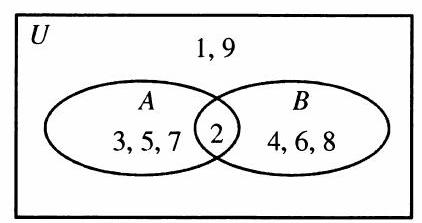
\includegraphics[width=0.5\textwidth]{images/2024_05_17_3b020e8fe1313185a92eg-014.jpg}
	\caption{维恩图的一个例子}
	\label{fig:Venn}
\end{figure}

\begin{example}
设 $A 、 B$ 都是不超过 9 的正整数组成的全集 $U$ 的子集, $A \cap B=$ $\{2\},\left(\complement_{U} A\right) \cap\left(\complement_{U} B\right)=\{1,9\},\left(\complement_{U} A\right) \cap B=\{4,6,8\}$, 求 $A \backslash B$.
\end{example}

\begin{analysis}
直接进行集合间的运算和推理似乎较难人手,但我们可从图\ref{fig:Venn}中得到解题思路的提示.
\end{analysis}

\begin{solution}
因为 $\complement_{U}(A \cup B)=\left(\complement_{U} A\right) \cap\left(\complement_{U} B\right)=$ $\{1,9\}$, 所以 $A \cup B=\{2,3,4,5,6,7,8\}$.

又

$$
\begin{aligned}
A \cap B & =\{2\}, \\
\left(\complement_{U} A\right) \cap B & =\{4,6,8\},
\end{aligned}
$$




所以

$$
\begin{aligned}
B & =U \cap B=\left(A \cup \complement_{U} A\right) \cap B \\
& =(A \cap B) \cup\left(\left(\complement_{U} A\right) \cap B\right) \\
& =\{2,4,6,8\} .
\end{aligned}
$$

所以, $A \backslash B=(A \cup B) \backslash B=\{3,5,7\}$.

\end{solution}

\begin{example}
已知集合 $A=\{(x, y) \mid a x+y=1\}, B=\{(x, y) \mid x+a y=1\}$, $C=\left\{(x, y) \mid x^{2}+y^{2}=1\right\}$. 问:

(1) 当 $a$ 取何值时, $(A \cup B) \cap C$ 为含有两个元素的集合?

(2) 当 $a$ 取何值时, $(A \cup B) \cap C$ 为含有三个元素的集合?

\end{example}

\begin{analysis}
因为 $(A \cup B) \cap C=(A \cap C) \cup(B \cap C)$, 故可从解 $A \cap C$ 及 $B \cap C$ 对应的方程组人手.
\end{analysis}

\begin{solution}
$(A \cup B) \cap C=(A \cap C) \cup(B \cap C), A \cap C$ 与 $B \cap C$ 分别为方程组

(i) $\left\{\begin{array}{l}a x+y=1, \\ x^{2}+y^{2}=1,\end{array}\right.$

(ii) $\left\{\begin{array}{l}x+a y=1, \\ x^{2}+y^{2}=1\end{array}\right.$
的解集.

由 (i) 解得 $(x, y)=(0,1),\left(\frac{2 a}{1+a^{2}}, \frac{1-a^{2}}{1+a^{2}}\right)$;

由 (ii) 解得 $(x, y)=(1,0),\left(\frac{1-a^{2}}{1+a^{2}}, \frac{2 a}{1+a^{2}}\right)$.

(1) 使 $(A \cup B) \cap C$ 恰有两个元素的情况只有两种可能:

(1) $\left\{\begin{array}{l}\frac{2 a}{1+a^{2}}=0, \\ \frac{1-a^{2}}{1+a^{2}}=1 ;\end{array}\right.$

(2) $\left\{\begin{array}{l}\frac{2 a}{1+a^{2}}=1 \\ \frac{1-a^{2}}{1+a^{2}}=0 .\end{array}\right.$\\
由(1)得 $a=0$; 由(2)得 $a=1$.

故当 $a=0$ 或 1 时, $(A \cup B) \cap C$ 恰有两个元素.

(2) 使 $(A \cup B) \cap C$ 恰有三个元素的情况是

$$
\frac{2 a}{1+a^{2}}=\frac{1-a^{2}}{1+a^{2}}
$$

解得 $a=-1 \pm \sqrt{2}$.

故当 $a=-1 \pm \sqrt{2}$ 时, $(A \cup B) \cap C$ 恰有三个元素.
\end{solution}

\begin{example}\label{ex:1.2.3}
设 $n \in \mathbf{N}$, 且 $n \geqslant 15, A 、 B$ 都是 $\{1,2, \cdots, n\}$ 的真子集, $A \cap B=\varnothing$,且 $\{1,2, \cdots, n\}=A \cup B$. 证明: $A$ 或者 $B$ 中必有两个不同数的和为完全平方数.
\end{example}

\begin{proof}
由题设, $\{1,2, \cdots, n\}$ 的任何元素必属于且只属于它的真子集 $A$ 、 $B$ 之一. 假设结论不真, 则存在如题设的 $\{1,2, \cdots, n\}$ 的真子集 $A 、 B$, 使得无论是 $A$ 还是 $B$ 中的任何两个不同的数的和都不是完全平方数.

不妨设 $1 \in A$, 则 $3 \notin A$. 否则 $1+3=2^{2}$, 与假设矛盾, 所以 $3 \in B$. 同样, $6 \notin B$, 所以 $6 \in A$. 这时 $10 \notin A$, 即 $10 \in B$. 因 $n \geqslant 15$, 而 15 或者在 $A$ 中, 或者在 $B$ 中,但当 $15 \in A$ 时, 因 $1 \in A, 1+15=4^{2}$, 矛盾; 当 $15 \in B$ 时,因 $10 \in B, 10+15=5^{2}$, 仍然矛盾. 因此假设不真, 即 $A$ 或者 $B$ 中必有两个不同数的和为完全平方数.
\end{proof}

\begin{note}
由 $A 、 B$ 地位对称, 在上面的解法中我们采用了“不妨设 $1 \in A$ ”这种技巧, 有效简化了解题过程.
\end{note}

例\ref{ex:1.2.3}实际上给出了一个关于集合的方程组:

$$
\left\{\begin{array}{l}
A \cup B=\{1,2, \cdots, n\} \\
A \cap B=\varnothing
\end{array}\right.
$$

如果交换 $A 、 B$ 算两组解 (有序解) ,那么这个方程组有多少组有序解呢?

设 $U=\{1,2, \cdots, n\}$, 由 $A \cup B=U, A \cap B=\varnothing$, 知 $A$ 与 $B$ 互补, 对于 $A \subseteq U$, 可取 $B=\complement_{U} A$. 故上述集合方程的有序解的个数为 $2^{n}$.

\begin{example}
设集合 $S$ 含有 $n$ 个元素, $A_{1}, A_{2}, \cdots, A_{k}$ 是 $S$ 的不同子集, 它们两两的交集非空, 而 $S$ 的其他子集不能与 $A_{1}, A_{2}, \cdots, A_{k}$ 都相交. 求证: $k=2^{n-1}$.
\end{example}

\begin{analysis}
$S$ 有 $2^{n}$ 个子集, 将两个互为补集的子集作为一组, 则可将 $2^{n}$ 个子集分成 $2^{n-1}$ 个组, 记为 $\left\{A_{i}^{\prime}, B_{i}^{\prime}\right\}, i=1,2, \cdots, 2^{n-1}$, 显然 $A_{i}$ 只能选取每组中的一个子集.
\end{analysis}

\begin{proof}
设 $a \in S$. 因为 $|S|=n$, 故 $S$ 的子集中含 $a$ 的子集有 $2^{n-1}$ 个. 显然\\
它们两两的交非空. 所以, $k \geqslant 2^{n-1}$.

又可将 $S$ 的 $2^{n}$ 个子集分成 $2^{n-1}$ 组, 每组有两个集合, 它们互为补集. 若 $k>2^{n-1}$, 则必有两个集合 $A_{i} 、 A_{j}(i \neq j)$ 来自上述同一组, 但 $A_{i} \cap A_{j}=\varnothing$, 与题意不符. 所以, $k=2^{n-1}$.
\end{proof}

\begin{example}
已知集合 $A$ 中包含 2016 个点且无四点共线. 证明: 在集合 $A$ 中存在一个至少有 63 个点的子集 $B$, 使得 $B$ 中无三点共线.
\end{example}

\begin{analysis}
自然,我们应该考虑集合 $A$ 中无三点共线的元素个数最多的子集, 设 $B$ 就是一个这样的子集, 那么集合 $A \backslash B$ 中任何一点都与集合 $B$ 中某两点构成三点共线,即 $A \backslash B$ 中任何一点对应集合 $B$ 中一个与之组成三点共线的二元子集, 且 $A \backslash B$ 中不同点对应 $B$ 中不同二元子集,故 $B$ 中二元子集的数量不少于 $A \backslash B$ 中元素的数量.
\end{analysis}

\begin{proof}
令 $B \subseteq A$ 且 $B$ 为无三点共线的最大的子集.

由于 $B$ 为满足条件的最大集合, 于是, 集合 $A \backslash B$ 中任意一点与集合 $B$ 中的某两个点共线.

又集合 $A$ 中无四点共线,则过集合 $B$ 中的两个点的每条直线最多包含集合 $A \backslash B$ 中的一个点.

故集合 $A \backslash B$ 中的点的数目不大于集合 $B$ 中的点对的数目.

记 $|B|=k$, 则集合 $A \backslash B$ 中点的数目为 $2016-k$, 集合 $B$ 中点对的数目为 $\frac{k(k-1)}{2}$. 所以

$$
2016-k \leqslant \frac{(k-1) k}{2}
$$

解得 $k \geqslant 63$ 或 $k \leqslant-64$ (负值舍去).

因此,集合 $B$ 中至少有 63 个点.
\end{proof}

\begin{example}
令 $S=\{1,2, \cdots, 2014\}$. 对于每个非空子集 $T \subseteq S$, 可选择 $T$ 的一个元素作为该集合的代表元. 求将集合 $S$ 的每个非空子集选取一个代表元的不同方式种数, 每种方式须满足对于每个子集 $D \subseteq S$, 若 $D$ 为非空子集 $A$, $B, C \subseteq S$ 的无交并(即子集 $A 、 B 、 C$ 两两不交且并集为 $D$ ), 则集合 $D$ 的代表元至少为 $A 、 B 、 C$ 中的一个代表元.
\end{example}

\begin{solution}
选取方式有 $108 \times 2014!$ 种.

用 $r(A)$ 表示集合 $A$ 的代表元, $a_{n}$ 表示当 $S=\{1,2, \cdots, n\}$ 时符合题意的安排方式的种数.

先计算四元集的情形.\\
记 $Y=\left\{y_{1}, y_{2}, y_{3}, y_{4}\right\}$. 则有四种不同方式选出 $r(Y)$, 不妨设 $y_{1}=$ $r(Y)$.

由 $\left\{y_{1}, y_{2}, y_{3}, y_{4}\right\}=\left\{y_{1}, y_{2}\right\} \cup\left\{y_{3}\right\} \cup\left\{y_{4}\right\}$, 则只能 $r\left(\left\{y_{1}, y_{2}\right\}\right)=$ $y_{1} \cdot$

类似地, $r\left(\left\{y_{1}, y_{3}\right\}\right)=r\left(\left\{y_{1}, y_{4}\right\}\right)=y_{1}$.

此时, 只有

$$
\begin{aligned}
& \left\{y_{1}, y_{2}, y_{3}\right\} 、\left\{y_{1}, y_{2}, y_{4}\right\} 、\left\{y_{1}, y_{3}, y_{4}\right\} 、 \\
& \left\{y_{2}, y_{3}, y_{4}\right\} 、\left\{y_{2}, y_{3}\right\} 、\left\{y_{2}, y_{4}\right\} 、\left\{y_{3}, y_{4}\right\}
\end{aligned}
$$

的代表元无法确定, 且可以为集合内的任意一个元素,故有 $3^{4} \times 2^{3}$ 种.

从而, $a_{4}=4 \times 3^{4} \times 2^{3}=108 \times 4!$.

对于 $n \geqslant 5$, 只要证明 $a_{n}=n a_{n-1}$.

记全集 $S$ 的代表元 $r(S)=k$, 则 $k$ 有 $n$ 种选择方式.

若 $T$ 为含 $k$ 的元素个数至多为 $n-2$ 的子集, 则集合 $S$ 可写成 $T$ 与另两个非空子集的无交并.

故 $r(T)=k$.

设 $T$ 为含 $k$ 的 $n-1$ 元子集.

若 $r(T)=m \neq k$, 则 $T$ 可写成 $\{m, k\}$ 与另两个子集的无交并.

从而, $r(\{m, k\})=m$, 这与之前的含 $k$ 的元素个数至多是 $n-2$ 的子集的代表元为 $k$ 的结论矛盾.

故含 $k$ 的所有子集代表元必为 $k$.

从而, 将 $n$ 降为了 $n-1$ 的情形可得递推式 $a_{n}=n a_{n-1}$.
\end{solution}

\begin{note}
正确理解集合 $D$ 的代表元的特殊性是解本例的关键. 设 $D=\left\{y_{1}\right.$, $\left.y_{2}, y_{3}, y_{4}\right\}, A=\left\{y_{1}, y_{2}\right\}, B=\left\{y_{3}\right\}, C=\left\{y_{4}\right\}$, 且 $r(A)=y_{1}$, 则 $D$ 的代表元不能为 $y_{2}$; 当然, 若 $r(A)=y_{2}$, 则 $D$ 的代表元不能为 $y_{1}$.
\end{note}

\begin{example}
有 1987 个集合,每个集合有 45 个元素,任意两个集合的并集有 89 个元素,问此 1987 个集合的并集有多少个元素?
\end{example}

\begin{analysis}
由每个集合有 45 个元素,且任意两个集合的并集有 89 个元素知,任意两个集合有且只有一个公共元素.
\end{analysis}

\begin{solution}
显然可以由题设找到这样的 1987 个集合, 它们都含有一个公共元素 $a$, 而且每两个集合不含 $a$ 以外的公共元素.

下面,我们来排除其他可能性.

由任意两个集合的并集有 89 个元素可知, 1987 个集合中的任意两个集合有且只有一个公共元素, 则容易证明这 1987 个集合中必有一个集合 $A$ 中\\
的元素 $a$ 出现在 $A$ 以外的 45 个集合中, 设为 $A_{1}, A_{2}, \cdots, A_{45}$, 其余的设为 $A_{46}, A_{47}, \cdots, A_{1986}$.

设 $B$ 为 $A_{46}, A_{47}, \cdots, A_{1986}$ 中的任一个集合, 且 $a \notin B$, 由题设 $B$ 和 $A$, $A_{1}, A_{2}, \cdots, A_{45}$ 都有一个公共元素, 且此 46 个元素各不相同, 故 $B$ 中有 46 个元素,与题设矛盾. 所以这 1987 个集合中均含有 $a$.

故所求结果为 $1987 \times 44+1=87429$,即这 1987 个集合的并集有 87429 个元素.
\end{solution}

\begin{note}
在这里我们先设计一种符合题设的特殊情形, 然后再排除其他可能的情形, 从而达到解题目的. 这是一种“先猜后证”的解题策略.
\end{note}

\begin{example}
将集合 $M=\{1,2, \cdots, 100\}$ 中任意 67 个数染成红色, 另 33 个数染成蓝色. 若集合 $M$ 存在形如

$$
A_{i, k}=\{i, i+1, \cdots, i+3 k-1\}(1 \leqslant k \leqslant 33,1 \leqslant i \leqslant 101-3 k)
$$

的子集恰有 $2 k$ 个数被染成红色, 另 $k$ 个数被染成蓝色, 求 $k$ 的最大值.
\end{example}

\begin{solution}
首先, 若将集合 $M$ 中从 $18 \sim 84$ 这 67 个数染成红色, 其他的数染成蓝色, 则当 $17<k \leqslant 33$ 时, 显然, 不存在满足题设条件的子集 $A_{i, k}$. 故 $k_{\max } \leqslant$ 17.

下面证明 $: k_{\text {max }}=17$.

事实上,当 $1 \leqslant i \leqslant 49$ 时,集合
$$
A_{i, 17}=\{i, i+1, \cdots, i+50\} \text { 与 } A_{i+1,17}=\{i+1, i+2, \cdots, i+51\}
$$

中红色数的个数至多相差 1.

(i) $i$ 与 $i+51$ 同色.

则集合 $A_{i, 17} 、 A_{i+1,17}$ 的红色数个数相等;

(ii) $i$ 为红、 $i+51$ 为蓝.

则集合 $A_{i, 17}$ 的红色数个数比集合 $A_{i+1,17}$ 的红色数个数多 1 ;

(iii) $i$ 为蓝、 $i+51$ 为红.

则集合 $A_{i, 17}$ 的红色数个数比集合 $A_{i+1,17}$ 的红色数个数少 1 .

考虑下面两个集合

$$
\begin{gathered}
A_{1,17}=\{1,2, \cdots, 51\} \\
A_{50,17}=\{50,51, \cdots, 100\}
\end{gathered}
$$

若 $A_{1,17} 、 A_{50,17}$ 中至少有一个集合恰好有 34 个数染成红色, 则结论成立.

设集合 $A_{1,17} 、 A_{50,17}$ 的红色数个数不是 34.\\
记 $A=A_{1,17} \cap A_{50,17}=\{50,51\}$.

下面分三种情形讨论.

(1)当集合 $A$ 中两个数均为红色时,由抽屉原则,知集合

$$
A_{1,17} \backslash A=\{1,2, \cdots, 49\} \text { 与 } A_{50,17} \backslash A=\{52,53, \cdots, 100\}
$$

中必有一个的红色数个数不少于 33.

由对称性, 不妨设集合 $A_{1,17} \backslash A$ 中的红色数个数不少于 33 , 则集合 $A_{1,17}$中的红色数个数不少于 35 ,集合 $A_{50,17}$ 中的红色数个数不多于 33.

由前面证明, 知集合 $A_{1.17}, A_{2,17}, \cdots, A_{50,17}$ 中至少有一个其红色数的个数恰为 33 .

(2) 当集合 $A$ 中两个数为 1 红 1 蓝时, 则集合 $A_{1,17} \backslash A$ 与 $A_{50,17} \backslash A$ 中红色数的个数一个多于 33 ,一个少于 33 . 同上可证.

(3) 当集合 $A$ 中两个数都为蓝色时, 则集合 $A_{1,17} \backslash A$ 与 $A_{50,17} \backslash A$ 中红色数的个数一个不少于 35, 一个不多于 33 . 同上可证.

综上, $k_{\max }=17$.
\end{solution}

\begin{example}
设 $m, n \in \mathbf{Z}_{+}$, 已知有 $n$ 堆金币,第 $i(1 \leqslant i \leqslant n)$ 堆中含有 $a_{i}\left(a_{i}>\right.$ 0) 枚. 鲍勃和爱丽丝按照如下步骤进行游戏:

【第一步】鲍勃选择集合 $\{1,2, \cdots, m\}$ 的非空子集 $B_{1}, B_{2}, \cdots, B_{n}$;

【第二步】在得知鲍勃第一步选择的集合 $B_{1}, B_{2}, \cdots, B_{n}$ 后, 爱丽丝选择集合 $\{1,2, \cdots, m\}$ 的一个非空子集 $S ;$

【第三步】若 $B_{i} \cap S$ 的元素个数为偶数, 则第 $i$ 堆的金币就归鲍勃所有,否则,归爱丽丝所有.

证明: 无论鲍勃如何选择集合 $B_{1}, B_{2}, \cdots, B_{n}$, 爱丽丝总能选择一个集合使得她得到的金币总数比鲍勃多.
\end{example}

\begin{proof}
游戏结束时, 爱丽丝获得的金币数多于鲍勃获得的金币数当且仅当

$$
\sum_{i=1}^{n}(-1)^{\left|B_{i} \cap S\right|} a_{i}<0
$$

否则,对任意的非空集合 $S$ 有

$$
\sum_{i=1}^{n}(-1)^{\left|B_{i} \cap S\right|} a_{i}>0
$$

显然, 当 $S=\varnothing$ 时,

$$
\sum_{i=1}^{n}(-1)^{\left|B_{i} \cap s\right|} a_{i}=\sum_{i=1}^{n} a_{i}>0
$$

故


\begin{equation*}
\sum_{S \subseteq\{1,2, \cdots, m\}} \sum_{i=1}^{n}(-1)^{\left|B_{i} \cap s\right|} a_{i}>0 \tag{1}
\end{equation*}


当 $B$ 是 $\{1,2, \cdots, m\}$ 的非空子集时, 考虑 $\sum_{S \subseteq\{1,2, \cdots, m\}}(-1)^{|B \cap S|}$.记 $S=C \cup D$, 其中, $C=S \backslash B, D=S \cap B, C \cap D=\varnothing$. 则

$$
\begin{aligned}
& \sum_{S \subseteq\{1,2, \ldots, m\}}(-1)^{|B \cap S|} \\
= & \sum_{C \subseteq\{1,2, \ldots, m \nmid B} \sum_{D \subseteq B}(-1)^{|B \cap(C U D)|} \\
= & \sum_{C \subseteq\{1,2, \cdots, m \backslash B} \sum_{D \subseteq B}(-1)^{|D|} .
\end{aligned}
$$

因为 $|B|>0$, 所以,

$$
\sum_{D \subseteq B}(-1)^{|D|}=\sum_{r=0}^{|B|}(-1)^{r} \mathrm{C}_{|B|}^{r}=0
$$

则对每个非空子集 $B \subseteq\{1,2, \cdots, m\}$ 有

$$
\sum_{S \subseteq\{1,2, \ldots, m\}}(-1)^{|B \cap S|}=0
$$

故

$$
\sum_{S \subseteq\{1,2, \ldots, m\}} \sum_{i=1}^{n}(-1)^{\left|B_{i} \cap S\right|} a_{i}=\sum_{i=1}^{n}\left[a_{i} \sum_{S \subseteq\{1,2, \ldots, m\}}(-1)^{\left|B_{i} \cap S\right|}\right]=0
$$

与式(1)矛盾.
\end{proof}

\begin{example}
设 $A$ 是集合 $S=\{1,2, \cdots, 1000000\}$ 的一个恰有 101 个元素的子集. 证明: 在 $S$ 中存在数 $t_{1}, t_{2}, \cdots, t_{100}$, 使得集合

$$
A_{j}=\left\{x+t_{j} \mid x \in A\right\}, j=1,2, \cdots, 100
$$

中,每两个的交集为空集.
\end{example}
\begin{analysis}
先弄清楚在什么情况下 $A_{i} \cap A_{j} \neq \varnothing$. 设 $a \in A_{i} \cap A_{j}$, 则 $a=x+$ $t_{i}=y+t_{j}, x, y \in A$. 于是 $t_{i}-t_{j}=y-x$. 这说明选取 $t_{1}, t_{2}, \cdots, t_{100}$ 时, 只要保证其中任意两个之差不等于 $A$ 中任二元素之差即可.
\end{analysis}

\begin{proof}
考虑集合 $D=\{x-y \mid x, y \in A\}$, 则

$$
|D| \leqslant 101 \times 100+1=10101
$$

若 $A_{i} \cap A_{j} \neq \varnothing$, 设 $a \in A_{i} \cap A_{i}$, 则 $a=x+t_{i}, a=y+t_{j}$, 其中 $x, y \in$ $A$,则 $t_{i}-t_{j}=y-x \in D$.

若 $t_{i}-t_{j} \in D$, 即存在 $x, y \in A$, 使得 $t_{i}-t_{j}=y-x$, 从而 $x+t_{i}=y+t_{j}$,即 $A_{i} \cap A_{j} \neq \varnothing$.

所以, $A_{i} \cap A_{j} \neq \varnothing$ 的充要条件是 $t_{i}-t_{j} \in D$. 于是, 我们只需在集 $S$ 中取出 100 个元素, 使得其中任意两个的差都不属于 $D$.

下面用递推方法来取出这 100 个元素.

先在 $S$ 中任取一个元素 $t_{1}$, 再从 $S$ 中取一个 $t_{2}$, 使得 $t_{1} \notin t_{2}+D=\left\{t_{2}+\right.$ $x \mid x \in D\}$, 这是因为取定 $t_{1}$ 后, 至多有 10101 个 $S$ 中的元素不能作为 $t_{2}$, 从而在 $S$ 中存在这样的 $t_{2}$, 若已有 $k(\leqslant 99)$ 个 $S$ 中的元素 $t_{1}, t_{2}, \cdots, t_{k}$ 满足要求, 再取 $t_{k+1}$, 使得 $t_{1}, t_{2}, \cdots, t_{k}$ 都不属于 $t_{k+1}+D=\left\{t_{k+1}+x \mid x \in D\right\}$. 这是因为 $t_{1}, t_{2}, \cdots, t_{k}$ 取定后, 至多有 $10101 k \leqslant 999999$ 个 $S$ 中的数不能作为 $t_{k+1}$,故在 $S$ 中存在满足条件的 $t_{k+1}$. 所以, 在 $S$ 中存在 $t_{1}, t_{2}, \cdots, t_{100}$, 其中任意两个的差都不属于 $D$.

综上所述, 命题得证.
\end{proof}

\begin{note}
条件 $|S|=10^{6}$ 可以改小一些. 一般地, 我们有如下更强的结论:

若 $A$ 是 $S=\{1,2, \cdots, n\}$ 的一个 $k$ 元子集, $m$ 为正整数,且 $m$ 满足条件 $n>(m-1)\left(\mathrm{C}_{k}^{2}+1\right)$, 则存在 $S$ 中的元素 $t_{1}, t_{2}, \cdots, t_{m}$, 使得 $A_{j}=\left\{x+t_{j} \mid\right.$ $x \in A\}, j=1,2, \cdots, m$ 中任意两个的交集为空集.

有兴趣者可自己证明.
\end{note}

\section{有限集的阶}
\section{子集族}
\section{集合的性质}
\section{集合中的最大(小)值}
\section{集合的分划}
\section{分类原则}
\section{极端原理}
\section{ 容斥原理}
\section{ 映射方法}